\documentclass[../main.tex]{subfiles}

\usepackage{makecell}
\usepackage{amsmath}

\titleformat{\section}
  {\normalsize\bfseries}{\thesection}{1em}{\normalfont}

\pagestyle{empty}

\setcounter{chapter}{4}
\pagenumbering{arabic}
\setcounter{page}{7}

\newenvironment{blockquote}{%
  \par%
  \medskip
  \leftskip=3.5em\rightskip=2em%
  \noindent\ignorespaces}{%
  \par\medskip}


\begin{document}

\chapter{}
\label{cha:cha_5}


\section{}
The function to evaluate is
\bigbreak
$f\left(c_{d}\right)=\sqrt{\dfrac{g m}{c_{d}}} \tanh \left(\sqrt{\dfrac{g c_{d}}{m}} t\right)-v(t)$
\bigbreak
or substituting the given values
\bigbreak
$f\left(c_{d}\right)=\sqrt{\dfrac{9.81(80)}{c_{d}}} \tanh \left(\sqrt{\dfrac{9.81 c_{d}}{80}} 4\right)-36$
\bigbreak
The first iteration is
\bigbreak
$x_{r}=\dfrac{0.1+0.2}{2}=0.15$
\bigbreak
$f(0.1) f(0.15)=0.860291(-0.204516)=-0.175944$
\bigbreak
Therefore, the root is in the first interval and the upper guess is redefined as $x_{u}=0.15$. The second iteration is
\bigbreak
$
\begin{aligned}
&x_{r}=\dfrac{0.1+0.15}{2}=0.125 \\\\
&\varepsilon_{a}=\left|\dfrac{0.125-0.15}{0.125}\right| 100 \%=20 \% \\\\
&f(0.1) f(0.125)=0.860291(0.318407)=0.273923
\end{aligned}
$
\bigbreak
Therefore, the root is in the second interval and the lower guess is redefined as $x_{u}=0.125$. 
\smallbreak
The remainder of the iterations are displayed in the following table:
\bigbreak
\begin{tabular}{|r|r|r|r|r|r|r|r|}
\hline
$i$ & $x_{l}$ & $f\left(x_{l}\right)$ & $x_{u}$ & $f\left(x_{u}\right)$ & $x_{r}$ & $f\left(x_{r}\right)$ & $\left|\varepsilon_{a}\right|$ \\
\hline
1 & $0.1$ & $0.86029$ & $0.2$ & $-1.19738$ & $0.15$ & $-0.20452$ &  \\
\hline
2 & $0.1$ & $0.86029$ & $0.15$ & $-0.20452$ & $0.125$ & $0.31841$ & $20.00 \%$ \\
\hline
3 & $0.125$ & $0.31841$ & $0.15$ & $-0.20452$ & $0.1375$ & $0.05464$ & $9.09 \%$ \\
\hline
4 & $0.1375$ & $0.05464$ & $0.15$ & $-0.20452$ & $0.14375$ & $-0.07551$ & $4.35 \%$ \\
\hline
5 & $0.1375$ & $0.05464$ & $0.14375$ & $-0.07551$ & $0.140625$ & $-0.01058$ & $2.22 \%$ \\
\hline
6 & $0.1375$ & $0.05464$ & $0.140625$ & $-0.01058$ & $0.1390625$ & $0.02199$ & $1.12 \%$ \\
\hline
\end{tabular}
\bigbreak
Thus, after six iterations, we obtain a root estimate of $\mathbf{0 . 1 3 9 0 6 2 5}$ with an approximate error of $1.12 \%$.
\bigbreak


\section{}
\begin{lstlisting}[numbers=none]
function root = bisectnew(func,xl,xu,Ead)
% bisectnew(xl,xu,es,maxit):
%   uses bisection method to find the root of a function
%   with a fixed number of iterations to attain
%   a prespecified tolerance
% input:
%   func = name of function
%   xl, xu = lower and upper guesses
%   Ead = (optional) desired tolerance (default = 0.000001)
% output:
%   root = real root

if func(xl)*func(xu)>0 %if guesses do not bracket a sign change
  error('no bracket') %display an error message and terminate
end
% if necessary, assign default values
if nargin<4, Ead = 0.000001; end %if Ead blank set to 0.000001
% bisection
xr = xl;
% compute n and round up to next highest integer
n = round(1 + log2((xu - xl)/Ead) + 0.5);
for i = 1:n
  xrold = xr;
  xr = (xl + xu)/2;
  if xr ~= 0, ea = abs((xr - xrold)/xr) * 100; end
  test = func(xl)*func(xr);
  if test < 0
 	  xu = xr;
  elseif test > 0
 	  xl = xr;
  else
    ea = 0;
  end
end
root = xr;
\end{lstlisting}
\bigbreak
The following is a MATLAB session that uses the function to solve Prob. 5.1 with $E_{a,d} = 0.0001.$
\bigbreak
\begin{lstlisting}[numbers=none]
>> fcd = inline('sqrt(9.81*80/cd)*tanh(sqrt(9.81*cd/80)*4)-36','cd')

fcd =
 Inline function:
 fcd(cd) = sqrt(9.81*80/cd)*tanh(sqrt(9.81*cd/80)*4)-36
 
>> format long
>> bisectnew(fcd,0.1,0.2,0.0001)

ans =
 0.14008789062500
\end{lstlisting}
\bigbreak

\section{}
The function to evaluate is
\bigbreak
$f\left(c_{d}\right)=\sqrt{\dfrac{9.81(80)}{C_{d}}} \tanh \left(\sqrt{\dfrac{9.81 c_{d}}{80}} 4\right)-36$
\bigbreak
The first iteration is
\bigbreak
$x_{r}=0.2-\dfrac{-1.19738(0.1-0.2)}{0.86029-(-1.19738)}=0.141809$
\bigbreak
$f(0.1) f(0.141809)=0.860291(-0.03521)=-0.030292$
\bigbreak
Therefore, the root is in the first interval and the upper guess is redefined as $X_{u}=0.141809$. 
\smallbreak
The second iteration is
\bigbreak
$x_{r}=0.141809-\dfrac{-0.03521(0.1-0.141809)}{0.86029-(-0.03521)}=0.140165$
\bigbreak
$\varepsilon_{a}=\left|\dfrac{0.140165-0.141809}{0.140165}\right| 100 \%=1.17 \%$
\bigbreak
Therefore, after only two iterations we obtain a root estimate of $0.140165$ with an\smallbreak approximate error of $1.17 \%$ which is below the stopping criterion of $2 \%$.
\bigbreak


\section{}
\begin{lstlisting}[numbers=none]
function root = falsepos(func,xl,xu,es,maxit)
% falsepos(xl,xu,es,maxit):
%   uses the false position method to find the root
%   of the function func
% input:
%   func = name of function
%   xl, xu = lower and upper guesses
%   es = (optional) stopping criterion (%) (default = 0.001)
%   maxit = (optional) maximum allowable iterations (default = 50)
% output:
%   root = real root
if func(xl)*func(xu)>0 %if guesses do not bracket a sign change
 error('no bracket') %display an error message and terminate
end
% default values
if nargin<5, maxit=50; end
if nargin<4, es=0.001; end
% false position
iter = 0;
xr = xl;
while (1)
  xrold = xr;
  xr = xu - func(xu)*(xl - xu)/(func(xl) - func(xu));
  iter = iter + 1;
  if xr ~= 0, ea = abs((xr - xrold)/xr) * 100; end
  test = func(xl)*func(xr);
  if test < 0
    xu = xr;
  elseif test > 0
    xl = xr;
  else
    ea = 0;
  end
  if ea <= es | iter >= maxit, break, end
end
root = xr;
\end{lstlisting}
 \bigbreak
 The following is a MATLAB session that uses the function to solve Prob. $5.1$ :
 \bigbreak
\begin{lstlisting}[numbers=none]
 >> fcd = inline('sqrt(9.81*80/cd)*tanh(sqrt(9.81*cd/80)*4)-36','cd')
 
fcd =
 Inline function:
 fcd(cd) = sqrt(9.81*80/cd)*tanh(sqrt(9.81*cd/80)*4)-36
 
>> format long
>> falsepos(fcd,0.1,0.2,2)

ans =
 0.14016503741282
\end{lstlisting}
 
 
\section{}
\textbf{Solve for the reactions:}

\bigbreak
$\mathrm{R}_{1}=265 \text { lbs. } \quad \mathrm{R}_{2}=285 \text { lbs. }$
\bigbreak

\textbf{Write beam equations:}
\bigbreak

$0<x<3 \hspace*{4cm} M+\left(16.667 x^{2}\right) \dfrac{x}{3}-265 x=0$
\bigbreak
\hspace*{5.2cm} $(1) \quad M=265-5.55 x^{3}$
\bigbreak
\bigbreak
$3<x<6 \hspace*{4cm} M+100(x-3)\left(\dfrac{x-3}{2}\right)+150\left(x-\dfrac{2}{3}(3)\right)-265 x=0$
\bigbreak
\hspace*{5.2cm} $(2)\quad M=-50 x^{2}+415 x-150$
\bigbreak
\bigbreak
$6<x<10 \hspace*{4.1cm}\ M=150\left(x-\dfrac{2}{3}(3)\right)+300(x-4.5)-265 x$
\bigbreak
\hspace*{5.2cm} $\quad(3)\quad M=-185 x+1650$
\bigbreak
\bigbreak
$10<x<12 \hspace*{4cm} M+100(12-x)=0$
\bigbreak
\hspace*{5.2cm} $\quad(4)\quad M=100 x-1200$
\bigbreak

\textbf{Combining Equations:}
\bigbreak
Because the curve crosses the axis between 6 and 10 , use (3).
\bigbreak
(3) $M=-185 x+1650$
\bigbreak
Set $x_{L}=6 ;\hspace*{0.15cm}	 x_{U}=10$ 
\bigbreak
$\begin{aligned}&M\left(x_{L}\right)=540 \\&M\left(x_{U}\right)=-200\end{aligned} \quad \quad\quad x_{r}=\dfrac{x_{L}+x_{U}}{2}=8$\smallbreak
$M\left(x_{R}\right)=170 \rightarrow$ replaces $x_{L}$
\bigbreak

$\begin{aligned}&M\left(x_{L}\right)=170 \\&M\left(x_{U}\right)=-200\end{aligned} \quad \quad\quad x_{r}=\dfrac{8+10}{2}=9$

$M\left(x_{R}\right)=-15 \rightarrow$ replaces $x_{U}$
\bigbreak

$\begin{aligned}&M\left(x_{\mathrm{L}}\right)=170 \\&M\left(x_{U}\right)=-15\end{aligned} \quad\quad\quad x_{r}=\dfrac{8+9}{2}=8.5$

$M\left(x_{R}\right)=77.5 \rightarrow$ replaces $x_{L}$
\bigbreak

$\begin{aligned}&M\left(x_{\mathrm{L}}\right)=77.5 \\&M\left(x_{U}\right)=-15\end{aligned} \quad\quad\quad x_{r}=\dfrac{8.5+9}{2}=8.75$

$M\left(x_{R}\right)=31.25 \rightarrow$ replaces $x_{L}$
\bigbreak

$\begin{aligned}&M\left(x_{\mathrm{L}}\right)=31.25 \\&M\left(x_{U}\right)=-15\end{aligned} \quad\quad\quad x_{r}=\dfrac{8.75+9}{2}=8.875$

$M\left(x_{R}\right)=8.125 \rightarrow$ replaces $x_{L}$
\bigbreak

$\begin{aligned}&M\left(x_{\mathrm{L}}\right)=8.125 \\&M\left(x_{U}\right)=-15\end{aligned} \quad\quad\quad x_{r}=\dfrac{8.875+9}{2}=8.9375$

$M\left(x_{R}\right)=-3.4375 \rightarrow$ replaces $x_{U}$
\bigbreak

$M\left(x_{\mathrm{L}}\right)=8.125$\\
$\hspace*{1.25cm}M\left(x_{U}\right)=-3.4375 \quad\quad\quad x_{r}=\dfrac{8.875+8.9375}{2}=8.90625$

$M\left(x_{R}\right)=2.34375 \rightarrow$ replaces $x_{L}$
\bigbreak

$\begin{aligned}&M\left(x_{\mathrm{L}}\right)=2.34375 \\&M\left(x_{U}\right)=-3.4375\end{aligned} \quad\quad\quad x_{r}=\dfrac{8.90625+8.9375}{2}=8.921875$

$M\left(x_{R}\right)=-0.546875 \rightarrow$ replaces $x_{U}$
\bigbreak

$M\left(x_{\mathrm{L}}\right)=2.34375$\\
	$\hspace*{1.25cm}M\left(x_{U}\right)=-0.546875 \quad\quad\quad x_{r}=\dfrac{8.90625+8.921875}{2}=8.9140625$
\bigbreak
$M\left(x_{\mathrm{R}}\right)=0.8984$ \textbf{Therefore}, $x=8.91$ feet
 \bigbreak
 
 
\section{}
\begin{enumerate}[label=\bfseries(\alph*)]
\item The graph can be generated with MATLAB
\bigbreak
\begin{lstlisting}[numbers=none] 
>> x=[-1:0.1:6];
>> f=-12-21*x+18*x.^2-2.75*x.^3;
>> plot(x,f)
>> grid 
\end{lstlisting}
\bigbreak
\begin{figure}[H]
		\hspace*{1.8cm}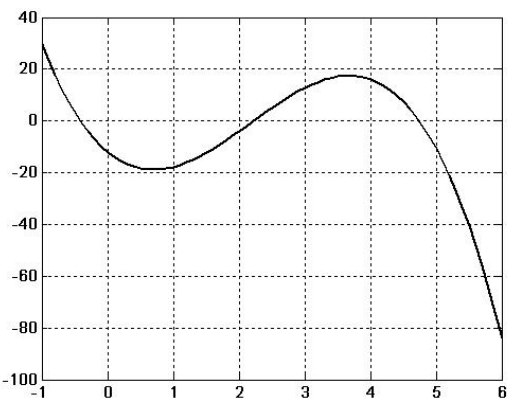
\includegraphics[width=0.5\linewidth]{fig_5_1}
		\label{fig:fig_5_1}
	\end{figure}
\bigbreak
This plot indicates that roots are located at about –$0.4, 2.25$ and $4.7$.
\bigbreak
\item Using bisection, the first iteration is
\bigbreak
$x_{r}=\dfrac{-1+0}{2}=-0.5$
\bigbreak
$f(-1) f(-0.5)=29.75(3.34375)=99.47656$
\bigbreak
Therefore, the root is in the second interval and the lower guess is redefined as $x_{l}=-0.5$.The \\second iteration is
\bigbreak
$x_{r}=\dfrac{-0.5+0}{2}=-0.25$
\bigbreak
$\varepsilon_{a}=\left|\dfrac{-0.25-(-0.5)}{-0.25}\right| 100 \%=100 \%$
\bigbreak
$f(-0.5) f(-0.25)=3.34375(-5.5820313)=-18.66492$
\bigbreak
Therefore, the root is in the first interval and the upper guess is redefined as $x_{u}=-0.25$. The \\remainder of the iterations are displayed in the following table:
\bigbreak

\begin{tabular}{|r|r|r|r|r|r|r|r|}
\hline
$i$ & $x_{l}$ & $f\left(x_{I}\right)$ & $x_{u}$ & $f\left(x_{u}\right)$ & $x_{r}$ & $f\left(x_{r}\right)$ & $\left|\varepsilon_{a}\right|$ \\
\hline
1 & $-1$ & $29.75$ & 0 & $-12$ & $-0.5$ & $3.34375$ &  \\
\hline
2 & $-0.5$ & $3.34375$ & 0 & $-12$ & $-0.25$ & $-5.5820313$ & $100.00 \%$ \\
\hline
3 & $-0.5$ & $3.34375$ & $-0.25$ & $-5.5820313$ & $-0.375$ & $-1.4487305$ & $33.33 \%$ \\
\hline
4 & $-0.5$ & $3.34375$ & $-0.375$ & $-1.4487305$ & $-0.4375$ & $0.8630981$ & $14.29 \%$ \\
\hline
5 & $-0.4375$ & $0.863098$ & $-0.375$ & $-1.4487305$ & $-0.40625$ & $-0.3136673$ & $7.69 \%$ \\
\hline
6 & $-0.4375$ & $0.863098$ & $-0.40625$ & $-0.3136673$ & $-0.421875$ & $0.2694712$ & $3.70 \%$ \\
\hline
7 & $-0.42188$ & $0.269471$ & $-0.40625$ & $-0.3136673$ & $-0.414063$ & $-0.0234052$ & $1.89 \%$ \\
\hline
8 & $-0.42188$ & $0.269471$ & $-0.41406$ & $-0.0234052$ & $-0.417969$ & $0.1227057$ & $0.93 \%$ \\
\hline
\end{tabular}
\bigbreak
Thus, after eight iterations, we obtain a root estimate of $\mathbf{- 0 . 4 1 7 9 6 9}$ with an approximate error of $0.93 \%$, which is below the stopping criterion of $1 \%$.
\bigbreak
\item Using false position, the first iteration is
\bigbreak
$x_{r}=0-\dfrac{-12(-1-0)}{29.75-(-12)}=-0.287425$
\bigbreak
$f(-1) f(-0.287425)=29.75(-4.4117349)=-131.2491$
\bigbreak
Therefore, the root is in the first interval and the upper guess is redefined as $X_{u}=-0.287425$.
\smallbreak
The second iteration is
\bigbreak
$x_{r}=-0.287425-\dfrac{-4.4117349(-1-(-0.287425))}{29.75-(-4.4117349)}=-0.3794489$
\bigbreak
$\varepsilon_{a}=\left|\dfrac{-0.3794489-(-0.2874251)}{-0.3794489}\right| 100 \%=24.25 \%$
\bigbreak
$f(-1) f(-0.3794489)=29.75(-1.2896639)=-38.3675$
\bigbreak
Therefore, the root is in the first interval and the upper guess is redefined as $x_{u}=-0.379449$.\\
The remainder of the iterations are displayed in the following table:
\bigbreak

\begin{tabular}{|r|r|r|r|r|r|r|r|}
\hline
$i$ & $x_{l}$ & $f\left(x_{l}\right)$ & $x_{u}$ & $f\left(x_{u}\right)$ & $x_{r}$ & $f\left(x_{r}\right)$ & $\left|\varepsilon_{a}\right|$ \\
\hline
1 & $-1$ & $29.75$ & 0 & $-12$ & $-0.287425$ & $-4.4117349$ &  \\
\hline
2 & $-1$ & $29.75$ & $-0.28743$ & $-4.4117349$ & $-0.379449$ & $-1.2896639$ & $24.25 \%$ \\
\hline
3 & $-1$ & $29.75$ & $-0.37945$ & $-1.2896639$ & $-0.405232$ & $-0.3512929$ & $6.36 \%$ \\
\hline
4 & $-1$ & $29.75$ & $-0.40523$ & $-0.3512929$ & $-0.412173$ & $-0.0938358$ & $1.68 \%$ \\
\hline
5 & $-1$ & $29.75$ & $-0.41217$ & $-0.0938358$ & $-0.414022$ & $-0.0249338$ & $0.45 \%$ \\
\hline
\end{tabular}
\bigbreak
Therefore, after five iterations we obtain a root estimate of $\mathbf{- 0 . 4 1 4 0 2 2}$ with an approximate \\error of $0.45 \%$, which is below the stopping criterion of $1 \%$.
\bigbreak


\section{}
A graph of the function can be generated with MATLAB
\bigbreak
\begin{lstlisting}[numbers=none]
>> x=[-0.5:0.1:1.5];
>> f=sin(x)-x.^2;
>> plot(x,f)
>> grid
\end{lstlisting}
\bigbreak
\begin{figure}[H]
		\hspace*{1.8cm}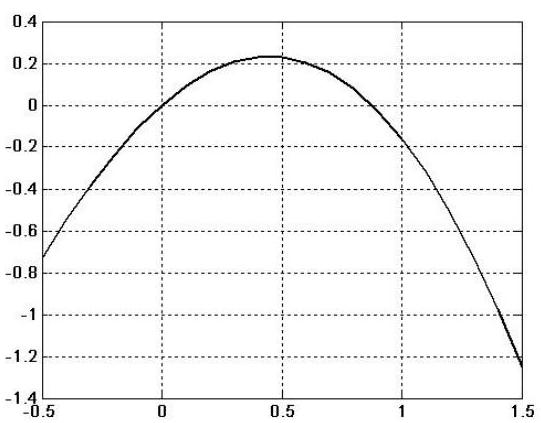
\includegraphics[width=0.5\linewidth]{fig_5_2}
		\label{fig:fig_5_2}
	\end{figure}
\bigbreak

This plot indicates that a nontrivial root (i.e., nonzero) is located at about $0.85$.
\bigbreak
Using bisection, the first iteration is
\bigbreak
$x_{r}=\dfrac{0.5+1}{2}=0.75$
\bigbreak
$f(0.5) f(0.75)=0.229426(0.1191388)=0.027333$
\bigbreak
Therefore, the root is in the second interval and the lower guess is redefined as $x_{l}=0.75$. The\\ second iteration is
\bigbreak
$x_{r}=\dfrac{0.75+1}{2}=0.875$
\bigbreak
$\varepsilon_{a}=\left|\dfrac{0.875-0.75}{0.875}\right| 100 \%=14.29 \%$
\bigbreak
$f(0.75) f(0.875)=0.119139(0.0019185)=0.000229$
\bigbreak
Because the product is positive, the root is in the second interval and the lower guess is\\ redefined as $x_{l}=0.875$. The remainder of the iterations are displayed in the following table:
\bigbreak

\begin{tabular}{|r|r|r|r|r|r|r|r|}
\hline
$i$ & $x_{l}$ & $f\left(x_{l}\right)$ & $x_{u}$ & $f\left(x_{u}\right)$ & $x_{r}$ & $f\left(x_{r}\right)$ & $\left|\varepsilon_{\mathrm{a}}\right|$ \\
\hline
1 & $0.5$ & $0.229426$ & 1 & $-0.158529$ & $0.75$ & $0.1191388$ &  \\
\hline
2 & $0.75$ & $0.119139$ & 1 & $-0.158529$ & $0.875$ & $0.0019185$ & $14.29 \%$ \\
\hline
3 & $0.875$ & $0.001919$ & 1 & $-0.158529$ & $0.9375$ & $-0.0728251$ & $6.67 \%$ \\
\hline
4 & $0.875$ & $0.001919$ & $0.9375$ & $-0.0728251$ & $0.90625$ & $-0.0340924$ & $3.45 \%$ \\
\hline
5 & $0.875$ & $0.001919$ & $0.90625$ & $-0.0340924$ & $0.890625$ & $-0.0157479$ & $1.75 \%$ \\
\hline
\end{tabular}
\bigbreak
Therefore, after five iterations we obtain a root estimate of $\mathbf{0 . 8 9 0 6 2 5}$ with an approximate error of $1.75 \%$, which is below the stopping criterion of $2 \%$.
\bigbreak
\end{enumerate}


\section{}
\begin{enumerate}[label=\bfseries(\alph*)]

\item A graph of the function indicates a positive real root at approximately $x=1.4$.
\bigbreak
\begin{figure}[H]
		\hspace*{0.4cm}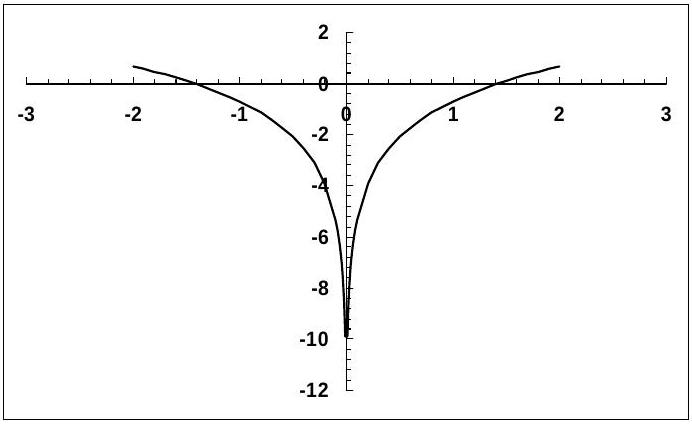
\includegraphics[width=0.7\linewidth]{fig_5_3}
		\label{fig:fig_5_3}
	\end{figure}
\bigbreak

\item Using bisection, the first iteration is
\bigbreak
$x_{r}=\dfrac{0.5+2}{2}=1.25$
\bigbreak
$f(0.5) f(1.25)=-2.08629(-0.2537129)=0.52932$
\bigbreak
Therefore, the root is in the second interval and the lower guess is redefined as $x_{l}=1.25$. The second iteration is
\bigbreak
$x_{r}=\dfrac{1.25+2}{2}=1.625$
\bigbreak
$\varepsilon_{a}=\left|\dfrac{1.625-1.25}{1.625}\right| 100 \%=23.08 \%$
\bigbreak
$f(1.25) f(1.625)=-0.253713(0.2710156)=-0.06876$
\bigbreak
Therefore, the root is in the first interval and the upper guess is redefined as $x_{u}=1.625$. The remainder of the iterations are displayed in the following table:
\bigbreak

\begin{tabular}{|r|r|r|r|r|r|r|r|}
\hline
$i$ & $x_{l}$ & $f\left(x_{l}\right)$ & $x_{u}$ & $f\left(x_{u}\right)$ & $x_{r}$ & $f\left(x_{r}\right)$ & $\left|\varepsilon_{a}\right|$ \\
\hline
1 & $0.5$ & $-2.08629$ & 2 & $0.6862944$ & $1.25$ & $-0.2537129$ &  \\
\hline
2 & $1.25$ & $-0.25371$ & 2 & $0.6862944$ & $1.625$ & $0.2710156$ & $23.08 \%$ \\
\hline
3 & $1.25$ & $-0.25371$ & $1.625$ & $0.2710156$ & $1.4375$ & $0.025811$ & $13.04 \%$ \\
\hline
\end{tabular}
\bigbreak
Thus, after three iterations, we obtain a root estimate of $\mathbf{1 . 4 3 7 5}$ with an approximate error of 13.04\%.
\bigbreak
\item Using false position, the first iteration is
\bigbreak
$
\begin{aligned}
&x_{r}=2-\dfrac{0.6862944(0.5-2)}{-2.086294-0.6862944}=1.628707 \\\\
&f(0.5) f(1.628707)=-2.086294(0.2755734)=-0.574927
\end{aligned}
$
\bigbreak
Therefore, the root is in the first interval and the upper guess is redefined as $x_{u}=1.628707$.\\ The second iteration is
\bigbreak
$
\begin{aligned}
&x_{r}=0.2755734-\dfrac{1.4970143(0.5-1.628707)}{-2.086294-0.2755734}=1.4970143 \\\\
&\varepsilon_{a}=\left|\dfrac{1.4970143-1.6287074}{1.4970143}\right| 100 \%=8.8 \% \\
\\&f(0.5) f(1.4970143)=-2.086294(0.1069453)=-0.223119
\end{aligned}
$
\bigbreak
Therefore, the root is in the first interval and the upper guess is redefined as $x_{u}=1.497014$.\\ The remainder of the iterations are displayed in the following table:
\bigbreak
\begin{tabular}{|r|r|r|r|r|r|r|r|}
\hline
$i$ & $x_{I}$ & $f\left(x_{I}\right)$ & $x_{u}$ & $f\left(x_{u}\right)$ & $x_{r}$ & $f\left(x_{r}\right)$ & $\left|\varepsilon_{a}\right|$ \\
\hline
1 & $0.5$ & $-2.08629$ & 2 & $0.6862944$ & $1.6287074$ & $0.2755734$ &  \\
\hline
2 & $0.5$ & $-2.08629$ & $1.628707$ & $0.2755734$ & $1.4970143$ & $0.1069453$ & $8.80 \%$ \\
\hline
3 & $0.5$ & $-2.08629$ & $1.497014$ & $0.1069453$ & $1.4483985$ & $0.040917$ & $3.36 \%$ \\
\hline
\end{tabular}
\bigbreak
Therefore, after three iterations we obtain a root estimate of $\mathbf{1 . 4 4 8 3 9 8 5}$ with an approximate error of $3.36 \%$.
\bigbreak
\end{enumerate}


\section{}
\begin{enumerate}[label=\bfseries(\alph*)]
\item Equation (5.6) can be used to determine the number of iterations
\bigbreak
$n=1+\log _{2}\left(\dfrac{\Delta x^{0}}{E_{a, d}}\right)=1+\log _{2}\left(\dfrac{35}{0.05}\right)=10.45121$
\bigbreak
which can be rounded up to 11 iterations.
\bigbreak

\begin{lstlisting}[numbers=none]
function TC = TempEval(osf)
% function to evaluate the temperature in degrees C based
% on the oxygen saturation concentration in freshwater (osf).
xl = 0 + 273.15;
xu = 35 + 273.15;
if fTa(xl,osf)*fTa(xu,osf)>0 %if guesses do not bracket
  error('no bracket') %display an error message and terminate
end
xr = xl;
for i = 1:11
  xrold = xr;
  xr = (xl + xu)/2;
  if xr ~= 0, ea = abs((xr - xrold)/xr) * 100; end
  test = fTa(xl,osf)*fTa(xr,osf);
  if test < 0
 	  xu = xr;
  elseif test > 0
 	  xl = xr;
  else
    ea = 0;
  end
end
TC = xr - 273.15;
end

function f = fTa(Ta, osf)
f = -139.34411 + 1.575701e5/Ta - 6.642308e7/Ta^2;
f = f + 1.2438e10/Ta^3 - 8.621949e11/Ta^4;
f = f - log(osf);
\end{lstlisting}
\bigbreak
The function can be used to evaluate the test cases:
\bigbreak
\begin{lstlisting}[numbers=none]

>> TempEval(8)

ans =
 26.7798
 
>> TempEval(10)

ans =
 15.3979
 
>> TempEval(14)

ans =
 1.5552

\end{lstlisting}
\end{enumerate}


\section{}
\begin{enumerate}[label=\bfseries(\alph*)]
\item The function to be evaluated is
\bigbreak
$f(y)=1-\dfrac{400}{9.81\left(3 y+y^{2} / 2\right)^{3}}(3+y)$
\bigbreak
A graph of the function indicates a positive real root at approximately $1.5 .$
\bigbreak
\begin{figure}[H]
		\hspace*{0.7cm}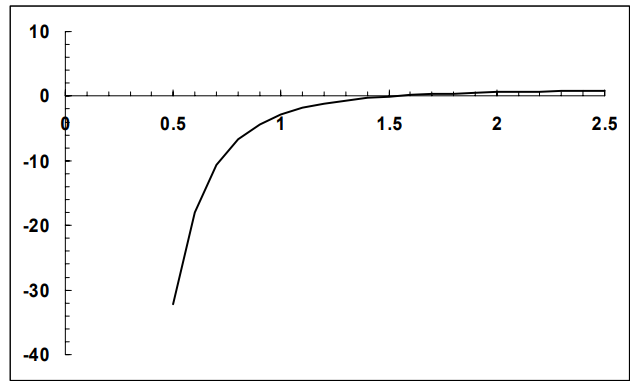
\includegraphics[width=0.6\linewidth]{fig_5_4}
		\label{fig:fig_5_4}
	\end{figure}
\bigbreak
\item Using bisection, the first iteration is
\bigbreak
$x_{r}=\dfrac{0.5+2.5}{2}=1.5$
\bigbreak
$f(0.5) f(1.5)=-32.2582(-0.030946)=0.998263$
\bigbreak
Therefore, the root is in the second interval and the lower guess is redefined as $x_{l}=1.5$. The second iteration is
\bigbreak
$x_{r}=\dfrac{1.5+2.5}{2}=2$
\bigbreak
$\varepsilon_{a}=\left|\dfrac{2-1.5}{2}\right| 100 \%=25 \%$
\bigbreak
$f(1.5) f(2)=-0.030946(0.601809)=-0.018624$
\bigbreak
Therefore, the root is in the first interval and the upper guess is redefined as $x_{u}=2$. The remainder of the iterations are displayed in the following table:
\bigbreak

\begin{tabular}{|r|r|r|r|r|r|r|r|}
\hline
$i$ & $x_{l}$ & $f\left(x_{l}\right)$ & $x_{u}$ & $f\left(x_{u}\right)$ & $x_{r}$ & $f\left(x_{r}\right)$ & $\left|\varepsilon_{a}\right|$ \\
\hline
1 & $0.5$ & $-32.2582$ & $2.5$ & $0.813032$ & $1.5$ & $-0.030946$ &  \\
\hline
2 & $1.5$ & $-0.03095$ & $2.5$ & $0.813032$ & 2 & $0.601809$ & $25.00 \%$ \\
\hline
3 & $1.5$ & $-0.03095$ & 2 & $0.601809$ & $1.75$ & $0.378909$ & $14.29 \%$ \\
\hline
4 & $1.5$ & $-0.03095$ & $1.75$ & $0.378909$ & $1.625$ & $0.206927$ & $7.69 \%$ \\
\hline
5 & $1.5$ & $-0.03095$ & $1.625$ & $0.206927$ & $1.5625$ & $0.097956$ & $4.00 \%$ \\
\hline
6 & $1.5$ & $-0.03095$ & $1.5625$ & $0.097956$ & $1.53125$ & $0.036261$ & $2.04 \%$ \\
\hline
7 & $1.5$ & $-0.03095$ & $1.53125$ & $0.036261$ & $1.515625$ & $0.003383$ & $1.03 \%$ \\
\hline
8 & $1.5$ & $-0.03095$ & $1.515625$ & $0.003383$ & $1.5078125$ & $-0.013595$ & $0.52 \%$ \\
\hline
\end{tabular}
\bigbreak
After eight iterations, we obtain a root estimate of $\mathbf{1 . 5 0 7 8 1 2 5}$ with an approximate error of $0.52 \% .$
\bigbreak

\item Using false position, the first iteration is
\bigbreak
$x_{r}=2.5-\dfrac{0.81303(0.5-2.5)}{-32.2582-0.81303}=2.45083$
\bigbreak
$f(0.5) f(2.45083)=-32.25821(0.79987)=-25.80248$
\bigbreak
Therefore, the root is in the first interval and the upper guess is redefined as $x_{u}=2.45083$. The second iteration is
\bigbreak
$x_{r}=2.45083-\dfrac{0.79987(0.5-2.45083)}{-32.25821-0.79987}=2.40363$
\bigbreak
$\varepsilon_{a}=\left|\dfrac{2.40363-2.45083}{2.40363}\right| 100 \%=1.96 \%$
\bigbreak
$f(0.5) f(2.40363)=-32.2582(0.78612)=-25.35893$
\bigbreak
The root is in the first interval and the upper guess is redefined as $x_{u}=2.40363$. The remainder of the iterations are displayed in the following table:
\bigbreak
\begin{tabular}{|r|r|r|r|r|r|r|r|}
\hline
$i$ & $x_{l}$ & $f\left(x_{l}\right)$ & $x_{u}$ & $f\left(x_{u}\right)$ & $x_{r}$ & $f\left(x_{r}\right)$ & $\left|\varepsilon_{a}\right|$ \\
\hline
1 & $0.5$ & $-32.2582$ & $2.50000$ & $0.81303$ & $2.45083$ & $0.79987$ &  \\
\hline
2 & $0.5$ & $-32.2582$ & $2.45083$ & $0.79987$ & $2.40363$ & $0.78612$ & $1.96 \%$ \\
\hline
3 & $0.5$ & $-32.2582$ & $2.40363$ & $0.78612$ & $2.35834$ & $0.77179$ & $1.92 \%$ \\
\hline
4 & $0.5$ & $-32.2582$ & $2.35834$ & $0.77179$ & $2.31492$ & $0.75689$ & $1.88 \%$ \\
\hline
5 & $0.5$ & $-32.2582$ & $2.31492$ & $0.75689$ & $2.27331$ & $0.74145$ & $1.83 \%$ \\
\hline
6 & $0.5$ & $-32.2582$ & $2.27331$ & $0.74145$ & $2.23347$ & $0.72547$ & $1.78 \%$ \\
\hline
7 & $0.5$ & $-32.2582$ & $2.23347$ & $0.72547$ & $2.19534$ & $0.70900$ & $1.74 \%$ \\
\hline
8 & $0.5$ & $-32.2582$ & $2.19534$ & $0.70900$ & $2.15888$ & $0.69206$ & $1.69 \%$ \\
\hline
9 & $0.5$ & $-32.2582$ & $2.15888$ & $0.69206$ & $2.12404$ & $0.67469$ & $1.64 \%$ \\
\hline
10 & $0.5$ & $-32.2582$ & $2.12404$ & $0.67469$ & $2.09077$ & $0.65693$ & $1.59 \%$ \\
\hline
\end{tabular}
\bigbreak

After ten iterations we obtain a root estimate of $\mathbf{2 . 0 9 0 7 7}$ with an approximate error of $1.59 \%$. Thus, after ten iterations, the false position method is converging at a very slow pace and is still far from the root in the vicinity of $1.5$ that we detected graphically.
\bigbreak
Discussion: This is a classic example of a case where false position performs poorly and is inferior to bisection. Insight into these results can be gained by examining the plot that was developed in part \textbf{(a)}. This function violates the premise upon which false position was based-that is, if $f\left(x_{u}\right)$ is much closer to zero than $f\left(x_{l}\right)$, then the root is closer to $x_{u}$ than to $x_{l}$ (recall Fig. 5.8). Because of the shape of the present function, the opposite is true.

\end{enumerate}
\end{document}

